\documentclass[10pt]{article}
\usepackage[letterpaper]{geometry}
\geometry{verbose,tmargin=1in,bmargin=1in,lmargin=1in,rmargin=1in}
\usepackage{setspace}
\usepackage{ragged2e}
\usepackage{color}
\usepackage{titlesec}
\usepackage{graphicx}
\usepackage{float}
\usepackage{mathtools}
\usepackage{amsmath}
\usepackage[font=small,labelfont=bf,labelsep=period]{caption}
\usepackage[english]{babel}
\usepackage{indentfirst}
\usepackage{array}
\usepackage{makecell}
\usepackage[usenames,dvipsnames]{xcolor}
\usepackage{multirow}
\usepackage{tabularx}
\usepackage{arydshln}
\usepackage{caption}
\usepackage{subcaption}
\usepackage{xfrac}
\usepackage{etoolbox}
\usepackage{cite}
\usepackage{url}
\usepackage{dcolumn}
\usepackage{hyperref}
\usepackage{courier}
\usepackage{url}
\usepackage{esvect}
\usepackage{commath}
\usepackage{verbatim} % for block comments
\usepackage{enumitem}
\usepackage{hyperref} % for clickable table of contents
\usepackage{braket}
\usepackage{titlesec}
\usepackage{booktabs}
\usepackage{gensymb}
\usepackage{longtable}
\usepackage{soul} % for striking out text
\usepackage[makeroom]{cancel}	% to cancel out text

\usepackage{listings}
\lstset{
    frame=single,
    breaklines=true,
    postbreak=\raisebox{0ex}[0ex][0ex]{\ensuremath{\color{red}\hookrightarrow\space}}
}

% for circled numbers
\usepackage{tikz}
\newcommand*\circled[1]{\tikz[baseline=(char.base)]{
            \node[shape=circle,draw,inner sep=2pt] (char) {#1};}}


\titleclass{\subsubsubsection}{straight}[\subsection]

% define new command for triple sub sections
\newcounter{subsubsubsection}[subsubsection]
\renewcommand\thesubsubsubsection{\thesubsubsection.\arabic{subsubsubsection}}
\renewcommand\theparagraph{\thesubsubsubsection.\arabic{paragraph}} % optional; useful if paragraphs are to be numbered

\titleformat{\subsubsubsection}
  {\normalfont\normalsize\bfseries}{\thesubsubsubsection}{1em}{}
\titlespacing*{\subsubsubsection}
{0pt}{3.25ex plus 1ex minus .2ex}{1.5ex plus .2ex}

\makeatletter
\renewcommand\paragraph{\@startsection{paragraph}{5}{\z@}%
  {3.25ex \@plus1ex \@minus.2ex}%
  {-1em}%
  {\normalfont\normalsize\bfseries}}
\renewcommand\subparagraph{\@startsection{subparagraph}{6}{\parindent}%
  {3.25ex \@plus1ex \@minus .2ex}%
  {-1em}%
  {\normalfont\normalsize\bfseries}}
\def\toclevel@subsubsubsection{4}
\def\toclevel@paragraph{5}
\def\toclevel@paragraph{6}
\def\l@subsubsubsection{\@dottedtocline{4}{7em}{4em}}
\def\l@paragraph{\@dottedtocline{5}{10em}{5em}}
\def\l@subparagraph{\@dottedtocline{6}{14em}{6em}}
\makeatother

\newcommand{\volume}{\mathop{\ooalign{\hfil$V$\hfil\cr\kern0.08em--\hfil\cr}}\nolimits}

\setcounter{secnumdepth}{4}
\setcounter{tocdepth}{4}
\begin{document}

\textbf{NE 255: HW5}1, 2\hfill April Novak\newline

\circled{1} The \(S_N\) form of the neutron transport equation is:

\begin{equation}
\label{eq:StartofOperatorForm}
\begin{aligned}
 \hat{\Omega}_a\cdot\nabla\psi_a^g(\vv{r}) + 
 \Sigma_t^g(\vv{r})\psi_a^g(\vv{r}) = \\
\sum_{l=0}^{N}\left\lbrack Y_{l0}^e(\hat{\Omega}_a)s_{l0}^g(\vv{r})+\sum_{m=1}^{l}\left(Y_{lm}^e(\hat{\Omega}_a)s_{lm}^g(\vv{r})+Y_{lm}^o(\hat{\Omega}_a)v_{lm}^g(\vv{r})\right)\right\rbrack+\\
\sum_{g'=1}^G\sum_{l=0}^{N}\Sigma_{s,l}(\vv{r}, g'\rightarrow g)\left\lbrack Y_{l0}^e(\hat{\Omega}_a)e_{l0}^{g'}(\vv{r})+\sum_{m=1}^{l}\left(Y_{lm}^e(\hat{\Omega}_a)e_{lm}^{g'}(\vv{r})+Y_{lm}^o(\hat{\Omega}_a)o_{lm}^{g'}(\vv{r})\right)\right\rbrack\quad\\
\end{aligned}
\end{equation}

The \(g\) superscript refers to the energy group number, and \(G\) to the total number of energy groups. Within-group scattering is counted in the scattering term, but is canceled by the total interaction term, which avoids double counting. The above equation can be cast in operator form. The external group source is defined as:

\begin{equation}
q_e^g(\vv{r})=\sum_{l=0}^{N}\left\lbrack Y_{l0}^e(\hat{\Omega}_a)s_{l0}^g(\vv{r})+\sum_{m=1}^{l}\left(Y_{lm}^e(\hat{\Omega}_a)s_{lm}^g(\vv{r})+Y_{lm}^o(\hat{\Omega}_a)v_{lm}^g(\vv{r})\right)\right\rbrack
\end{equation}

in order to permit easier equation manipulation. In addition, several operators are defined. The transport operator is:

\begin{equation}
\textbf{L}\equiv\hat{\Omega}_a\cdot\nabla+\Sigma_t^g
\end{equation}

and the solution vector \(\Psi\) is a column vector containing each energy group flux vector \(\vv{\psi}\):

\begin{equation}
\Psi=\begin{bmatrix}\vv{\psi}_1&\vv{\psi}_2&\vv{\psi}_3&\cdots&\vv{\psi}_G\end{bmatrix}^T
\end{equation}

where \(\vv{\psi}\) is then a column vector that contains the flux for each discrete angle for that particular energy group \(g\):

\begin{equation}
\vv{\psi}_g=\begin{bmatrix}\psi_1^g&\psi_2^g&\psi_3^g&\cdots&\psi_n^g\end{bmatrix}^T
\end{equation}

So, the vector of unknowns is organized by energy group, and in the section pertaining to each group, by angle. In order to discuss the size of these matrices and vectors, several variables are defined:

\begin{equation}
\begin{aligned}
G=&\ \text{number of energy groups}\\
t = &\ \text{number of moments}\\
n = &\ \text{number of angles}\\
N = &\ P_N\text{\ order}\\
N_c=&\ \text{number of cells}\\
N_e=&\ \text{number of unknowns per cell}\\
\end{aligned}
\end{equation} 

So, if the problem consisted of a single cell with a single node (i.e. only one spatial unknown), then \(\Psi\) would be an \((Gn)\times1\) vector. However, the problems solves will consist of a spatial domain that is also present in \(\Psi\). In reality, each \(\psi_{\hat{\Omega}_n}^g\) term is solved as a function of space, and is therefore not a scalar value, but an \(N_cN_e\times1\) vector. The \(S_N\) equation for a particular angle and group is solved as a function of space using a variety of methods, such as the finite element method or the finite difference method. So, the total size of \(\Psi\) is \(N_cN_eGn\times1\). The external source \(q_e^g\) is defined in a similar manner, and is represented as \(Q\), an \(N_cN_eGn\times1\) vector.

Expressing the mapping between flux moments and the scattering term is more difficult simply due to the difficulty in visualizing the matrix multiplication. The moment-to-discrete matrix is used to project harmonic moments onto discrete angle space. It is defined as:

\begin{equation}
\textbf{M}=\left\{
\begin{array}{*{13}c}
Y_{00}^o(\hat{\Omega}_1) & Y_{00}^e(\hat{\Omega}_1) & Y_{01}^o(\hat{\Omega}_1) & Y_{01}^e(\hat{\Omega}_1) & Y_{10}^o(\hat{\Omega}_1) & Y_{10}^e(\hat{\Omega}_1) & Y_{11}^o(\hat{\Omega}_1) & Y_{11}^e(\hat{\Omega}_1) & \cdots & Y_{NN}^o(\hat{\Omega}_1) & Y_{NN}^e(\hat{\Omega}_1)\\
Y_{00}^o(\hat{\Omega}_2) & Y_{00}^e(\hat{\Omega}_2) & Y_{01}^o(\hat{\Omega}_2) & Y_{01}^e(\hat{\Omega}_2) & Y_{10}^o(\hat{\Omega}_2) & Y_{10}^e(\hat{\Omega}_2) & Y_{11}^o(\hat{\Omega}_2) & Y_{11}^e(\hat{\Omega}_2) & \cdots & Y_{NN}^o(\hat{\Omega}_2) & Y_{NN}^e(\hat{\Omega}_2)\\
\vdots & \vdots & \vdots & \vdots & \vdots & \vdots & \vdots & \vdots & \vdots & \vdots & \vdots \\
Y_{00}^o(\hat{\Omega}_n) & Y_{00}^e(\hat{\Omega}_n) & Y_{01}^o(\hat{\Omega}_n) & Y_{01}^e(\hat{\Omega}_n) & Y_{10}^o(\hat{\Omega}_n) & Y_{10}^e(\hat{\Omega}_n) & Y_{11}^o(\hat{\Omega}_n) & Y_{11}^e(\hat{\Omega}_n) & \cdots & Y_{NN}^o(\hat{\Omega}_n) & Y_{NN}^e(\hat{\Omega}_n)\\
\end{array}\right\}
\end{equation}

But, some of these components are actually always zero - for instance, from the expansion in Eq. \eqref{eq:StartofOperatorForm}, if \(l=0\), then there are no spherical harmonics for which \(m\neq0\). This eliminates \(Y_{01}^e\) and \(Y_{01}^o\). In addition, \(Y_{00}^o=0\) and \(Y_{10}^o=0\) since there is no odd component for \(m=0\). This gives a simplified version of the moment-to-discrete matrix, where the only difference between this matrix and the more explicit one above is that several of the low \(l\) and \(m\) spherical harmonics that are zero are removed.

\begin{equation}
\textbf{M}=\left\{
\begin{array}{*{13}c}
Y_{00}^e(\hat{\Omega}_1)  & Y_{10}^e(\hat{\Omega}_1) & Y_{11}^o(\hat{\Omega}_1) & Y_{11}^e(\hat{\Omega}_1) & Y_{20}^e(\hat{\Omega}_1) & \cdots & Y_{NN}^o(\hat{\Omega}_1) & Y_{NN}^e(\hat{\Omega}_1)\\
Y_{00}^e(\hat{\Omega}_2)  & Y_{10}^e(\hat{\Omega}_2) & Y_{11}^o(\hat{\Omega}_2) & Y_{11}^e(\hat{\Omega}_2) & Y_{20}^e(\hat{\Omega}_2) & \cdots & Y_{NN}^o(\hat{\Omega}_2) & Y_{NN}^e(\hat{\Omega}_2)\\
\vdots & \vdots & \vdots & \vdots & \vdots & \vdots & \vdots & \vdots \\
Y_{00}^e(\hat{\Omega}_n) & Y_{10}^e(\hat{\Omega}_n) & Y_{11}^o(\hat{\Omega}_n) & Y_{11}^e(\hat{\Omega}_n) & Y_{20}^e(\hat{\Omega}_n) & \cdots & Y_{NN}^o(\hat{\Omega}_n) & Y_{NN}^e(\hat{\Omega}_n)\\
\end{array}\right\}
\end{equation}

The scattering matrix contains along its diagonal the scattering moments:

\begin{equation}
\textbf{S}_{g^{'}\rightarrow g}=\begin{bmatrix}
\Sigma_{s0}
\end{bmatrix}
\end{equation}

With this definition, the discretization of the transport equation leads to the following matrix system:

\begin{equation}
\textbf{L}\begin{bmatrix}\Psi_1\\\Psi_2\\\Psi_3\\\vdots\\\Psi_G\end{bmatrix}=
\begin{bmatrix}
\textbf{M} & 0 & 0 & 0 & 0\\
0 & \textbf{M} & 0 & 0 & 0\\
0 & 0 & \textbf{M} & 0 & 0\\
0 & 0 & 0 & \cdots & 0\\
0 & 0 & 0 & 0 & \textbf{M}\\
\end{bmatrix}
\begin{bmatrix}
\textbf{S}_{11} & \textbf{S}_{12} & \textbf{S}_{13} & \cdots & \textbf{S}_{1G}\\
\textbf{S}_{21} & \textbf{S}_{22} & \textbf{S}_{23} & \cdots & \textbf{S}_{2G}\\
\textbf{S}_{31} & \textbf{S}_{32} & \textbf{S}_{33} & \cdots & \textbf{S}_{3G}\\
\vdots & \vdots & \vdots & \vdots & \vdots\\
\textbf{S}_{G1} & \textbf{S}_{G2} & \textbf{G}_{23} & \cdots & \textbf{S}_{GG}\\
\end{bmatrix}
\begin{bmatrix}
\Phi_1\\\Phi_2\\\Phi_3\\\vdots\\\Phi_G
\end{bmatrix}
+
\begin{bmatrix}
Q_1\\Q_2\\Q_3\\\vdots\\Q_G
\end{bmatrix}
\end{equation}

Hence, the upper triangular portion of the scattering matrix represents upscattering, while the diagonal represents within-group scattering, and the lower triangular portion represents downscattering. \(\Phi\) represents a vector of the angular flux moments used in the expansion of the scattering term, organized by group. 

\begin{equation}
\Phi_g=\begin{bmatrix}
o_{00}^g & e_{00}^g & o_{01}^g & e_{01}^g & o_{10}^g & e_{10}^g & \cdots & o_{NN}^g & e_{NN}^g\\
\end{bmatrix}^T
\end{equation}

where \(e_{lm}\) and \(o_{lm}\) are defined by Eq. \eqref{eq:FluxMoments31}. Note, however, that some of these terms are zero due to how the expansion is performed. Moments with \(l=0\) are only nonzero for \(m=0\). And, there is no odd component for \(l=0\). 

\begin{equation}
\Phi_g=\begin{bmatrix}
e_{00}^g & e_{10}^g & o_{11}^g & e_{11}^g & \cdots & o_{NN}^g & e_{NN}^g\\
\end{bmatrix}^T
\end{equation}

\begin{equation}
\label{eq:FluxMoments31}
\begin{aligned}
e_{lm}(\vv{r},E')=\int_{4\pi}^{}d\hat{\Omega}'Y_{lm}^e(\hat{\Omega}')\psi(\vv{r}, E',\hat{\Omega}')\\
o_{lm}(\vv{r},E')=\int_{4\pi}^{}d\hat{\Omega}'Y_{lm}^o(\hat{\Omega}')\psi(\vv{r}, E',\hat{\Omega}')\\
\end{aligned}
\end{equation}

For this specific problem, the discretized \(S_N\) equations become:

\begin{equation}
\label{eq:MatrixEquationProblem1}
\underbrace{\textbf{L}}_{\circled{1}}\underbrace{\begin{bmatrix}\Psi_1\\\Psi_2\\\Psi_3\\\end{bmatrix}}_{\circled{2}}=
\underbrace{\begin{bmatrix}
\textbf{M} & 0 & 0 \\
0 & \textbf{M} & 0 \\
0 & 0 & \textbf{M} \\
\end{bmatrix}}_{\circled{3}}
\underbrace{\begin{bmatrix}
\textbf{S}_{11} & \textbf{S}_{12} & \textbf{S}_{13} \\
\textbf{S}_{21} & \textbf{S}_{22} & \textbf{S}_{23} \\
\textbf{S}_{31} & \textbf{S}_{32} & \textbf{S}_{33} \\
\end{bmatrix}}_{\circled{4}}
\underbrace{\begin{bmatrix}
\Phi_1\\\Phi_2\\\Phi_3
\end{bmatrix}}_{\circled{5}}
+
\underbrace{\begin{bmatrix}
Q_1\\Q_2\\Q_3
\end{bmatrix}}_{\circled{6}}
\end{equation}

where the groups are numbered 1, 2, and 3, with 1 being the highest-energy group.\newline

\textbf{(a)}: The dimensions of each of the matrices shown in Eq. \eqref{eq:MatrixEquationProblem1} are summarized in the table below, according to the numbering scheme shown above. For this problem, \(G=3, n=8, N_c=4^3, N_e=4, N=2, t=(N+1)^2=9\). \(N_e=4\) because for each cell, the cell-centered flux and the outgoing fluxes for three of the six faces are unknown.

\begin{table}[h]
\caption{Sizes of matrices in Eq. \eqref{eq:MatrixEquationProblem1}.}
\centering
\begin{tabular}{c c c}
\hline\hline
Matrix or Vector & Size (Symbolic) & Size (Actual) \\ [0.5ex]
\hline % inserts single-line
\circled{1} & \(GnN_cN_e\times GnN_cN_e\) & \(6144\times6144\)\\
\circled{2} & \(GnN_cN_e\times1\) & \(6144\times1\)\\
\circled{3} & \(GnN_cN_e\times GtN_cN_e\) & \(6144\times6192\)\\
\circled{4} & \(GtN_cN_e\times GtN_cN_e\) & \(6192\times6192\)\\
\circled{5} & \(GtN_cN_e\times 1\) & \(6192\times1\)\\
\circled{6} & \(GnN_cN_e\times1\) & \(6144\times1\)\\
\hline
\end{tabular}
\end{table}

\textbf{(b)}: For this particular problem:

\begin{equation}
\textbf{M}_{gg}=\left\{
\begin{array}{*{13}c}
Y_{00}^e(\hat{\Omega}_1)  & Y_{10}^e(\hat{\Omega}_1) & Y_{11}^o(\hat{\Omega}_1) & Y_{11}^e(\hat{\Omega}_1) & Y_{20}^e(\hat{\Omega}_1) & Y_{21}^o(\hat{\Omega}_1) & Y_{21}^e(\hat{\Omega}_1) & Y_{22}^o(\hat{\Omega}_1) & Y_{22}^e(\hat{\Omega}_1)\\
Y_{00}^e(\hat{\Omega}_2)  & Y_{10}^e(\hat{\Omega}_2) & Y_{11}^o(\hat{\Omega}_2) & Y_{11}^e(\hat{\Omega}_2) & Y_{20}^e(\hat{\Omega}_2) & Y_{21}^o(\hat{\Omega}_2) & Y_{21}^e(\hat{\Omega}_2) & Y_{22}^o(\hat{\Omega}_2) & Y_{22}^e(\hat{\Omega}_2)\\
Y_{00}^e(\hat{\Omega}_3)  & Y_{10}^e(\hat{\Omega}_3) & Y_{11}^o(\hat{\Omega}_3) & Y_{11}^e(\hat{\Omega}_3) & Y_{20}^e(\hat{\Omega}_3) & Y_{21}^o(\hat{\Omega}_3) & Y_{21}^e(\hat{\Omega}_3) & Y_{22}^o(\hat{\Omega}_3) & Y_{22}^e(\hat{\Omega}_3)\\
Y_{00}^e(\hat{\Omega}_4)  & Y_{10}^e(\hat{\Omega}_4) & Y_{11}^o(\hat{\Omega}_4) & Y_{11}^e(\hat{\Omega}_4) & Y_{20}^e(\hat{\Omega}_4) & Y_{21}^o(\hat{\Omega}_4) & Y_{21}^e(\hat{\Omega}_4) & Y_{22}^o(\hat{\Omega}_4) & Y_{22}^e(\hat{\Omega}_4)\\
Y_{00}^e(\hat{\Omega}_5)  & Y_{10}^e(\hat{\Omega}_5) & Y_{11}^o(\hat{\Omega}_5) & Y_{11}^e(\hat{\Omega}_5) & Y_{20}^e(\hat{\Omega}_5) & Y_{21}^o(\hat{\Omega}_5) & Y_{21}^e(\hat{\Omega}_5) & Y_{22}^o(\hat{\Omega}_5) & Y_{22}^e(\hat{\Omega}_5)\\
Y_{00}^e(\hat{\Omega}_6)  & Y_{10}^e(\hat{\Omega}_6) & Y_{11}^o(\hat{\Omega}_6) & Y_{11}^e(\hat{\Omega}_6) & Y_{20}^e(\hat{\Omega}_6) & Y_{21}^o(\hat{\Omega}_6) & Y_{21}^e(\hat{\Omega}_6) & Y_{22}^o(\hat{\Omega}_6) & Y_{22}^e(\hat{\Omega}_6)\\
Y_{00}^e(\hat{\Omega}_7)  & Y_{10}^e(\hat{\Omega}_7) & Y_{11}^o(\hat{\Omega}_7) & Y_{11}^e(\hat{\Omega}_7) & Y_{20}^e(\hat{\Omega}_7) & Y_{21}^o(\hat{\Omega}_7) & Y_{21}^e(\hat{\Omega}_7) & Y_{22}^o(\hat{\Omega}_7) & Y_{22}^e(\hat{\Omega}_7)\\
Y_{00}^e(\hat{\Omega}_8)  & Y_{10}^e(\hat{\Omega}_8) & Y_{11}^o(\hat{\Omega}_8) & Y_{11}^e(\hat{\Omega}_8) & Y_{20}^e(\hat{\Omega}_8) & Y_{21}^o(\hat{\Omega}_8) & Y_{21}^e(\hat{\Omega}_8) & Y_{22}^o(\hat{\Omega}_8) & Y_{22}^e(\hat{\Omega}_8)\\
\end{array}\right\}
\end{equation}

Then, matrix \circled{3} is assembled by aligning these \(\textbf{M}\) matrices along the diagonal, as shown in Eq. \eqref{eq:MatrixEquationProblem1}. The scattering matrix \(\textbf{S}\) is comprised of scattering matrices \(\textbf{S}_{gg^{'}}\), and is shown in Eq. \eqref{eq:MatrixEquationProblem1}. One of these scattering matrices is, for example:

\begin{equation}
\textbf{S}_{21}=\begin{bmatrix}
\Sigma_{s0}^{21} & 0 & 0 & 0 & 0 & 0 & 0 & 0 & 0\\
0& \Sigma_{s1}^{21}  & 0 & 0 & 0 & 0 & 0 & 0 & 0\\
0& 0 & \Sigma_{s1}^{21}  & 0 & 0 & 0 & 0 & 0 & 0\\
0& 0 & 0 & \Sigma_{s1}^{21}  & 0 & 0 & 0 & 0 & 0\\
0& 0 & 0 & 0 & \Sigma_{s2}^{21}  & 0 & 0 & 0 & 0\\
0& 0 & 0 & 0 & 0 & \Sigma_{s2}^{21}  & 0 & 0 & 0\\
0& 0 & 0 & 0 & 0 & 0 & \Sigma_{s2}^{21}  & 0 & 0\\
0& 0 & 0 & 0 & 0 & 0 & 0 & \Sigma_{s2}^{21} & 0\\
0& 0 & 0 & 0 & 0 & 0 & 0 & 0 & \Sigma_{s2}^{21}\\
\end{bmatrix}
\end{equation}

The vector of unknowns is:

\begin{equation}
\Psi=\begin{bmatrix}\Psi_1 & \Psi_2 & \Psi_3\end{bmatrix}
\end{equation}

where, for example, 

\begin{equation}
\Psi_1=\begin{bmatrix}\psi_1^1 & \psi_2^1 & \psi_3^1 & \psi_4^1 & \psi_5^1 & \psi_6^1 & \psi_7^1 & \psi_8^1
\end{bmatrix}
\end{equation}

where the subscripts indicates the angle, and the superscript indicates the energy group. The vector of flux moments is:

\begin{equation}
\Phi=\begin{bmatrix}\Phi_1 & \Phi_2 & \Phi_3\end{bmatrix}
\end{equation}

where, for example,

\begin{equation}
\Phi_1=\begin{bmatrix}
e_{00}^1 & e_{10}^1 & o_{11}^1 & e_{11}^1 & e_{20}^1 & o_{21}^1 & e_{21}^1 & o_{22}^1 & e_{22}^1
\end{bmatrix}^T
\end{equation}

where the superscript indicates the energy group. The moments \(e\) and \(o\) are defined in Eq. \eqref{eq:FluxMoments31}.\newline

\textbf{(c)}: The \textbf{D} matrix is used to convert between the discrete angular fluxes to the moments of the angular flux by \(\phi=\textbf{D}\psi\). The discrete form of \textbf{D} is defined by:

\begin{equation}
\textbf{D}=\textbf{M}^T\textbf{W}
\end{equation}

where \textbf{M} is defined in Eq. \eqref{eq:MatrixEquationProblem1} as containing \(\textbf{M}_{gg}\) matrices along its diagonal and \textbf{W} is a diagonal matrix containing \(n\) quadrature points per group (since we're using \(S_N\)) - these quadrature points are aligned along the diagonal in a repeated fashion for each energy group. The form of \textbf{D} is therefore:

\begin{equation}
\textbf{D}=\begin{bmatrix}
w_1Y_{00}^e & w_2Y_{00}^e & w_3Y_{00}^e & w_4Y_{00}^e & w_5Y_{00}^e & w_6Y_{00}^e & w_7Y_{00}^e & w_8Y_{00}^e\\
w_1Y_{10}^e & w_2Y_{10}^e & w_3Y_{10}^e & w_4Y_{10}^e & w_5Y_{10}^e & w_6Y_{10}^e & w_7Y_{10}^e & w_8Y_{10}^e\\
w_1Y_{11}^o & w_2Y_{11}^o & w_3Y_{11}^o & w_4Y_{11}^o & w_5Y_{11}^o & w_6Y_{11}^o & w_7Y_{11}^o & w_8Y_{11}^o\\
w_1Y_{11}^e & w_2Y_{11}^e & w_3Y_{11}^e & w_4Y_{11}^e & w_5Y_{11}^e & w_6Y_{11}^e & w_7Y_{11}^e & w_8Y_{11}^e\\
w_1Y_{20}^e & w_2Y_{20}^e & w_3Y_{20}^e & w_4Y_{20}^e & w_5Y_{20}^e & w_6Y_{20}^e & w_7Y_{20}^e & w_8Y_{20}^e\\
w_1Y_{21}^o & w_2Y_{21}^o & w_3Y_{21}^o & w_4Y_{21}^o & w_5Y_{21}^o & w_6Y_{21}^o & w_7Y_{21}^o & w_8Y_{21}^o\\
w_1Y_{21}^e & w_2Y_{21}^e & w_3Y_{21}^e & w_4Y_{21}^e & w_5Y_{21}^e & w_6Y_{21}^e & w_7Y_{21}^e & w_8Y_{21}^e\\
w_1Y_{22}^o & w_2Y_{22}^o & w_3Y_{22}^o & w_4Y_{22}^o & w_5Y_{22}^o & w_6Y_{22}^o & w_7Y_{22}^o & w_8Y_{22}^o\\
w_1Y_{22}^e & w_2Y_{22}^e & w_3Y_{22}^e & w_4Y_{22}^e & w_5Y_{22}^e & w_6Y_{22}^e & w_7Y_{22}^e & w_8Y_{22}^e\\
\end{bmatrix}
\end{equation}

\textbf{(d)}: Because the matrices involved in only this \(4\times4\) mesh are relatively large, none of them are directly formed so that zero entries do not need to be stored. Instead, all matrix-matrix or matrix-vector products are performed according to their indices. For instance, to multiply a \(n\times1\) vector \(V\) by a \(n\times n\) matrix \(M\) to give a resulting vector \(r\), each component of \(r\) would be dictated by:

\begin{equation}
r_i=\sum_{j=1}^nM_{ij}V_j
\end{equation}

and so on for the matrix multiplication. Avoiding storage of the matrices is a huge advantage, since a majority of their contents are zero anyways, and for iterative solution methods, it is common practice to take advantage of the fact that the matrix does not need to be performed to further reduce the runtime.\newline

\textbf{(e)}: To get a matrix system entirely in terms of \(\Psi\), begin with the operator form:

\begin{equation}
\textbf{L}\Psi=\textbf{M}\textbf{S}\Phi+\textbf{M}q_e
\end{equation}

and insert \(\Psi=\textbf{D}\Phi\). This can transform the above equation either into an equation for \(\Phi\) or \(\Psi\). I'm not sure which approach is done in practice, so I'll write both forms:

\begin{equation}
\textbf{L}\textbf{D}\Phi=\textbf{M}\textbf{S}\Phi+\textbf{M}q_e\quad\rightarrow\quad(\textbf{L}\textbf{D}-\textbf{M}\textbf{S})\Phi=\textbf{M}q_e
\end{equation}

And for the equation in terms of \(\Psi\):

\begin{equation}
\textbf{L}\Psi=\textbf{M}\textbf{S}\textbf{D}^{-1}\Psi+\textbf{M}q_e\quad\rightarrow\quad(\textbf{L}-\textbf{M}\textbf{S}\textbf{D}^{-1})\Psi=\textbf{M}q_e
\end{equation}

\circled{2}: This question implements a Jacobi solver to create a multigroup transport solver using the Weighted Diamond Difference (WDD) code developed from the previous assignment. This code from the previous assignment is used to perform the within-group solves for the angular flux in the \(\pm0.2,\pm0.5,\pm0.7\) directions. Within each of these iterations, the scattering source within each group (angle to angle) is iteratively updated. Then, outside of each within-group calculation, the overall group source is updated. I assume that the right boundary condition is kept as a reflective boundary condition, since this was performed in the previous assignment (and we're not given a condition there). I also assumed that the incoming flux for group 1 was evenly split amongst the three different angles. The group source is updated according to:

\begin{equation}
\text{group source}=\sum_{g^{'}=1}^G\Sigma_s(g^{'}\rightarrow g)\psi_{g^{'}}
\end{equation}

using the same set of quadrature rules as from the previous assignment (note: not a real quadrature set, but am using this from the previous assignment). Fig. \ref{fig:1} shows the scalar fluxes obtained using this multigroup solver. 

\begin{figure}[H]
  \centering
  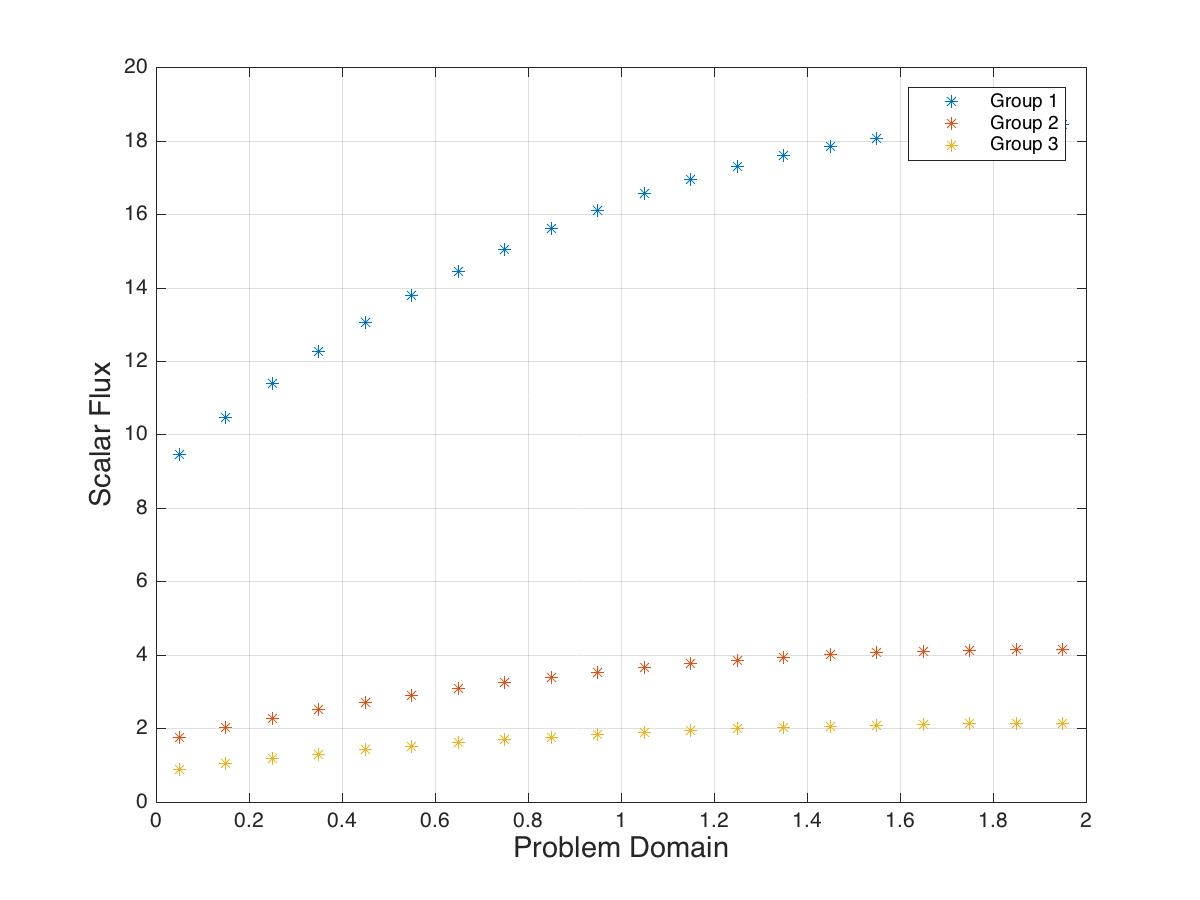
\includegraphics[width=12cm]{ScalarFlux_3Group.jpg} % versioned
  \caption{Scalar flux for the three energy groups.}
  \label{fig:1}
\end{figure}

\section{Appendix}
This section contains all the code used for each question. 

\subsection{Question 2}
\lstinputlisting[language=Matlab]{Q2.m}


\end{document}